\chapter{Optimizaciones estructurales}
	
Un algoritmo con buenos resultados visuales viene con unos costes computacionales asociados. A parte de buscar fotorrealismo y fidelidad gráfica, un motor de renderizado gráfico requiere de mejoras y optimizaciones para alcanzar tiempos competentes.

La importancia de las optimizaciones implementadas en este capítulo no solo se limita a mejorar la productividad de los artistas con mejoras de rendimiento, si no que hace posible la visualización real de escenas que tardarían tiempos del orden de miles de años, reduciendo el enfoque de fuerza bruta a uno más sofisticado.
	
\section{Muestreo por importancia}
\label{sec:mi}

El simple hecho de simular los caminos de los fotones no es eficiente. Se puede buscar una manera para que cada camino cargue con información ''más útil''. Este procedimiento se denomina ''Muestreo por importancia'' y es actualmente una línea de investigación en constante desarrollo ya que como se verá a continuación, permite mejoras muy significativas en cuanto al tiempo de convergencia de la imagen final.

Gran parte de la literatura al respecto se resume en las notas de Importance Sampling for Production Rendering\cite{colbert2010importance} donde se repasan todos los fundamentos teóricos del muestreo por importancia. Así pues en este trabajo solo se va a ofrecer una visión generalizada suficiente para entender la implementación realizada en Eleven Renderer.

Esta implementación consta de tres muestreos por importancia distintos: Muestreo por importancia de BRDF, Estimación de Evento Próximo (NEE) y Muestreo por importancia del mapa de entorno.

Algo que todas las técnicas de  muestreo por importancia tienen en común es su funcionamiento primario: Emitir más rayos en las direcciones que más interesan y a su vez, dividir el resultado por la función de distribución de probabilidad (\code{pdf} en adelante). Esto quiere decir que si se emiten el doble de rayos en una dirección que en otra, será necesario dividir este resultado por dos, puesto que se ha recabado el doble de radiación lumínica. Así pues, también se tendrá que multiplicar el resultado menos muestreado por el doble, ya que al muestrear la mitad, se obtiene la mitad de radiación.

Cuando se ha explicado \hyperref[subsec:montecarlo]{la aproximación de la Ecuación de Renderizado} se ha mostrado un denominador $p(\omega _{\text{k}})$ que hasta el momento no ha jugado ningún papel. Este denominador es en efecto la función \code{pdf}.

En la implementación, todo muestreo consiste en una función que genera rayos aleatorios a aquellos lugares donde interesa más muestrear \code{sample()} y la función de distribución de probabilidad apropiada \code{pdf()} derivada de la función de muestreo, que ha de devolver la probabilidad con la que se ha elegido ese camino. Como se verá más adelante, no siempre es fácil derivar esta función de probabilidad cuando se cuenta con una función de muestreo compleja.


\subsection{Muestreo por importancia de entorno}
	
Anteriormente se ha descrito como la iluminación HDRI permite resultados visualmente complejos de manera sencilla, simplemente una imagen con alta profundidad de color. Este método por otra parte también cuenta con inconvenientes. 

Antes de aplicar cualquier tipo de optimización a este método de iluminación, se estaba trazando un rayo de manera ingenua, recibiendo el color de la imagen a partir de las coordenadas esféricas asumiendo una esfera de radio infinito. Para imágenes homogéneas con luminosidad similar en cada píxel, este método funciona muy bien, pero la mayoría de estas imágenes HDRI consisten en un paisaje con componentes lumínicos condensados tales como el sol el cual actúa como principal fuente de luz.

Esta situación plantea un problema, y es que los focos de luz como puede ser el sol, concentran un gran porcentaje de luminosidad, mientras que el resto de la imagen no. Esto implica que pocas veces se va a recibir información del sol, lo que va a resultar en ''fireflies''. La forma de enfrentar este problema es igual que el resto de muestreo por importancia: Trazar más rayos a los píxeles más luminosos, ya que serán aquellos que más información aporten a la escena.

La implementación de este tipo de muestreo por importancia no es trivial. Las imágenes HDRI utilizadas normalmente en la industria cinematográfica suelen contar con resoluciones extremas (~8K) y son del orden de millones de píxeles. La búsqueda de los píxeles más brillantes y la asignación de su probabilidad de ser elegidos requerirá de un preprocesamiento previo que facilite dicha búsqueda.

El planteamiento general para este método consiste en precomputar un array del tamaño del número total de píxeles de la imagen HDRI, en el que cada elemento cuente con la iluminación acumulada normalizada hasta el momento de cada píxel.
La función que determina la iluminación de un píxel viene dada por la respuesta logarítmica media de los bastones y conos de los ojos para cada longitud de onda, pero para simplificar se utilizará la suma de cada componente de color. Este array a efectos prácticos contiene la función de distribución acumulativa discreta normalizada (CDF) y además como está ordenado, es posible hacer búsquedas binarias, las cuales cuentan con una complejidad logarítmica (aproximadamente 25 iteraciones de búsqueda para una imagen de 8K de resolución).

Así pues, si se quiere obtener un píxel de manera aleatoria proporcional a su iluminación, bastará con buscar en el CDF el intervalo que comprende el valor aleatorio dado. Esta operación de búsqueda también tiene coste logarítmico, ya que es una versión ligeramente modificada de la búsqueda binaria corriente.


\begin{figure}[H]
    \centering
	\includegraphics[width=0.5\textwidth]{CDF}
	\caption{División BVH}
	\label{fig:label}
\end{figure}


La función de distribución de probabilidad pdf vendrá entonces dada por la iluminación para el pixel obtenido dividida por la iluminación total.


\subsection{Muestreo por importancia de Estimación de Evento Próximo (NEE)}



El renderizado por luz directa es un método por el cual solo se tiene en cuenta la primera interacción del rayo con la escena y se comprueba si dicho punto es visible a los elementos lumínicos. Este método converge muy rápido puesto que solo necesita computar una interacción y el fotón recibe información directamente de la luz sin tener que desperdiciar fotones que acaben en zonas oscuras, pero carece del fotorrealismo que ofrece la iluminación global o luz indirecta, puesto no tiene en cuenta la luz reflejada en otros elementos no emisivos.

El muestreo por importancia de Estimación de Evento Próximo trata de juntar estos dos métodos: La iluminación directa y la indirecta. De esta manera, la parte expuesta directamente a elementos lumínicos convergerá rápidamente, además de las partes afectadas por la iluminación global, que lo harán también. Un añadido de este método es la posibilidad de computar la iluminación dada por luces de punto.

Las luces de punto consisten en un punto en el espacio infinitamente pequeño el cual emite luz de manera uniforme hacia todos los lados. Sin la implementación de la estimación de evento próximo, estas luces al ser infinitesimalmente pequeñas, jamás serían alcanzadas por los fotones y por lo tanto, nunca se recibiría información de ellas. No solo eso, NEE también permite una mejor convergencia en las luces de menor tamaño, puesto que originalmente, las luces tienen menos probabilidades de ser alcanzadas cuanto menor sea su área.


\subsection{Muestreo por importancia de BRDF}

La función BRDF aporta distintas intensidades lumínicas dependiendo de la dirección entrante y la dirección saliente, así pues sería mucho más óptimo lanzar más rayos a los sitios en los que esta función sea mayor e ignorar aquellos sitios donde no se aporte mucha información al resultado final.

Un ejemplo que ayuda a visualizar este caso son los materiales perfectamente reflectantes, (espejos). Los materiales reflectantes tienen un valor BRDF = 1 para todo rayo entrante simétrico al saliente con la normal como eje de reflexión. Para el resto de direcciones, el valor será 0. Así pues, no tiene sentido emitir rayos aleatorios donde se conozca que el resultado del BRDF será 0.

Otro ejemplo es el muestreo por coseno. La ecuación de renderizado cuenta con un término que pondera radiación obtenida por el modelo BRDF a partir del coseno del ángulo incidente. Por esta razón, tiene sentido emitir de manera proporcional a este término más rayos allá donde el coseno es más grande.

\subsection{Muestreo por importancia múltiple:}

El muestreo por importancia es una herramienta que mejora considerablemente los tiempos de convergencia en determinados escenarios, aunque la verdadera utilidad de estos es elegir el muestreo correcto para cada situación. En 1975 se propone una técnica conocida como MIS (Multiple Importance Sampling). Esta técnica evaluará todas las funciones de  muestreo para cada intersección y dará mayor importancia con un escalar a aquellas funciones que proporcionen mayor información de la escena.

(AÑADIR TEORÏA AQUÍ)







\section{Estructuras de aceleración}
\label{BVH}
	
Pese a que este punto cuenta con un nombre genérico, las estructuras de aceleración en el ámbito del renderizado por trazado de rayos hacen referencia a la interacción específica entre geometrías tridimensionales y los rayos generados por la cámara. La intersección Rayo-Triángulo no es en sí una operación demandante a nivel computacional, pero la mayoría de las escenas suelen contar con complejas geometrías del orden de miles de millones de triángulos.

El enfoque más ingenuo y utilizado hasta el momento en este motor de renderizado consiste en evaluar triángulo a triángulo si intersecciona con el rayo dado. Así pues, se observa que es posible reducir el número de comprobaciones de intersecciones aplicando una jerarquía espacial a los triángulos, que descarte parte de ellos para cada interacción, reduciendo así considerablemente el número de operaciones.

Existen diversas formas de estructurar estas jerarquías. Nombrando las más conocidas: Octrees, k-d tree y BVH. En esta implementación se ha usado BVH puesto que se considera que tiene muy buenos resultados.

BVH es acrónimo de "Bounding Volume Hierarchy", traducido como jerarquía del volumen delimitador y consiste en un árbol binario de profundidad definida en el que cada nodo cuenta con un el prisma rectangular que delimita un conjunto de triángulos (en la práctica este prisma consiste en dos puntos en el espacio). Cada nodo interior tiene dos hijos y cada hijo, el volumen delimitador del subconjunto disjunto de los triángulos del nodo padre. Los nodos hoja cuentan con el volumen delimitador y con una lista de los triángulos que contienen.

\begin{figure}
    \centering
	\includegraphics[width=0.5\textwidth]{BVH}
	\caption{División BVH}
	\label{fig:label}
\end{figure}

De esta manera será posible descartar gran parte de los triángulos comprobando los volúmenes por los cuales interseccionan los rayos.

Esta nueva estructura de datos BVH cuenta con dos operaciones fundamentales: La operación de creación \code{build} y la operación de recorrido \code{transverse}. La operación de creación será necesaria solo una vez al principio de cada renderizado de escena y podrá ser realizada en la CPU para mayor simplicidad. La operación de recorrido sin embargo será ejecutada cada vez que se quiera comprobar la interacción Rayo-Triángulo.

El algoritmo empleado es una interpretación del libro PBRT, pero difiere en varios detalles. Pharr et al. \cite{pharr2016physically} almacena un solo triángulo por cada nodo hoja, a diferencia del código implementado en Eleven Renderer, donde hay una profundidad máxima definida como \code{BVH\_DEPTH}, y los nodos hojas almacenan los índices de uno o varios triángulos. 

\subsection{Operación de generación de BVH (CPU)}

La operación de generación parte de la generación recursiva de un árbol binario por profundidad, añadiendo información adicional a los nodos.

\begin{enumerate}
	
\item Para cada nodo que contiene un conjunto de triángulos, se calcula el volumen delimitador. Este volumen viene dado por el vértice menor y mayor del volumen \code{b1, b2}.

\item Se separa el conjunto de triángulos en dos subconjuntos disjuntos. El cómo se divide este conjunto se delega a la función \code{divideSAH()}, que hará uso de la heurística de superficie de área para decidir qué triángulos van a cada subconjunto.

\item Finalmente se aplica recursión para los hijos generados en caso de residir en un nodo interior, o se termina la recursión y se almacenan los índices \code{from} y \code{to} de los triángulos que estos contienen en caso de ser un nodo hoja.

\end{enumerate}

Los delimitadores son dos puntos que representan el volumen que contiene una geometría. El cálculo de estos se hace cogiendo las coordenadas mínimas y máximas. La operación de unión de estos delimitadores se hace aplicando el mismo esquema de coordenadas mínimas y máximas.

\begin{lstlisting}
	
	void buildAux(int depth, std::vector<BVHTri>* _tris) {

		Vector3 b1, b2;

		if (depth == 0)
			totalTris = _tris->size();

		if(depth == 7)
			printf("\rAllocated tris: %d / %d, %d%%", allocatedTris, totalTris, (100 * allocatedTris) / totalTris);

		bounds(_tris, b1, b2);

		if (depth == DEPTH) {

			nodes[nodeIdx++] = Node(nodeIdx, b1, b2, triIdx, triIdx + _tris->size(), depth);

			for (int i = 0; i < _tris->size(); i++)
				triIndices[triIdx++] = _tris->at(i).index;

			allocatedTris += _tris->size();
		}
		else {

			nodes[nodeIdx++] = Node(nodeIdx, b1, b2, 0, 0, depth);

			std::vector<BVHTri>* trisLeft = new std::vector<BVHTri>();
			std::vector<BVHTri>* trisRight = new std::vector<BVHTri>();

			divideSAH(_tris, trisLeft, trisRight);

			buildAux(depth + 1, trisLeft);
			buildAux(depth + 1, trisRight);

			trisLeft->clear();
			trisRight->clear();

			delete trisLeft;
			delete trisRight;
		}
	}
	
\end{lstlisting}

Una duda que puede surgir es cómo se almacenan los triángulos de manera eficiente en estos árboles, ya que almacenar tantas listas como nodos hoja hay, es muy ineficiente en términos de memoria. Aquí es donde entran en juego los índices \code{from} y \code{to} mencionados anteriormente. Se hace uso de una lista de ordenación de triángulos denominada \code{triIndices}, la cual contiene índices de los triángulos en la lista original ordenados por nodos. Los nodo hoja tendrán pues dos índices indicando desde qué índice (\code{from}) hasta qué índice (\code{to}) es necesario leer de manera inclusiva en esta lista para recuperar los triángulos almacenados por dicho nodo.

\begin{figure}[H]
    \centering
	\includegraphics[width=0.5\textwidth]{triIndices}
	\caption{triIndices}
	\label{fig:label}
\end{figure}

Una vez definida la función de generación de árboles BVH solo queda decidir cómo se van a particionar los triángulos en cada nodo.

El hecho de como separar los nodos hijos de manera óptima no es una tarea trivial, en esta sección se mostrarán comparativas mostrando como los tiempos de recorrido varían dependiendo del método elegido, además de que algunos métodos tardan más en construirse pero permiten recorridos más rápidos mientras que otros métodos permiten la construcción de árboles en tiempo lineal pero no ofrecen tan buenos resultados a la hora de recorrerlos. Estos últimos son más usados en aplicaciones de tiempo real que requieren construir árboles BVH en milisegundos.

La aplicación de este trabajo requiere de varios segundos e incluso minutos por cada escena renderizada, por lo que existe la libertad de construir árboles con métodos más lentos que no afectarán tan negativamente al tiempo total de renderizado.

Se han implementado dos métodos distintos para comparar su rendimiento. Uno de ellos es un método ingenuo y el segundo es un método utilizado en producción conocido como división por heurística de superficie (SAH).

\subsubsection{Partición por plano:}

En el libro Physically based rendering: From theory to implementation \cite{pharr2016physically} se propone un método de partición sencillo. A continuación se explica una interpretación algo distinta de este método que hace uso de los centroides de los triángulos en vez de utilizar el vértice 0 como hace el libro.

Este método no es práctico y se usa tan solo de forma comparativa. Consiste en elegir la dimensión más grande de la caja que envuelve a los triángulos y partirla por la mitad. Posteriormente se recorrerán todos los triángulos y se dividirán por dicho plano. Para saber si un triángulo se encuentra a un lado o al otro se interpretan los triángulos como un punto en el espacio cuya posición es el centroide.

\begin{lstlisting}
	
	static void dividePlane(std::vector<BVHTri>* tris, std::vector<BVHTri>* trisLeft, std::vector<BVHTri>* trisRight) {

		Vector3 b1, b2;

		bounds(tris, b1, b2);

		Vector3 l = (b2.x - b1.x, b2.y - b1.y, b2.z - b1.z);

		if (l.x > l.y && l.x > l.z) {

			for (int i = 0; i < tris->size(); i++) {
				if (tris->at(i).tri.centroid().x > b1.x + l.x / 2) {
					trisLeft->push_back(tris->at(i));
				}
				else {
					trisRight->push_back(tris->at(i));
				}
			}

		} else if (l.y > l.x && l.y > l.z) {
			for (int i = 0; i < tris->size(); i++) {
				if (tris->at(i).tri.centroid().y > b1.y + l.y / 2) {
					trisLeft->push_back(tris->at(i));
				}
				else {
					trisRight->push_back(tris->at(i));
				}
			}
		}
		else {
			for (int i = 0; i < tris->size(); i++) {
				if (tris->at(i).tri.centroid().z > b1.z + l.z / 2) {
					trisLeft->push_back(tris->at(i));
				}
				else {
					trisRight->push_back(tris->at(i));
				}
			}
		}
	}
	
\end{lstlisting}

\subsubsection{Heurística SAH:}
	

\subsection{Operación de recorrido (GPU)}
	
El recorrido de árboles es una tarea intuitivamente recursiva y cuenta con una implementación conocida y sencilla. No obstante la recursión es un proceso indeseado en CUDA debido a las pilas relativamente pequeñas de los dispositivos de aceleración gráfica. Así pues también generan una divergencia superior, un proceso con alta penalización en el rendimiento.

Para demostrar esto se ha hecho uso de dos implementaciones de la función de recorrido. La primera es una función recursiva de recorrido de árboles binarios:

\begin{lstlisting}
	
	__host__ __device__ void transverseAux(Ray ray, Hit& nearestHit, Node& node) {
	
		if (node.depth == BVH_DEPTH) {
			intersectNode(ray, node, nearestHit);
			return;
		}
	
		Node lChild = leftChild(node.idx, node.depth);
		Node rChild = rightChild(node.idx, node.depth);
	
		if (intersect(ray, lChild.b1, lChild.b2))
			transverseAux(ray, nearestHit, lChild);
		
		if (intersect(ray, rChild.b1, rChild.b2))
			transverseAux(ray, nearestHit, rChild);		
	}

\end{lstlisting}

	
Karras explica en el blog de desarrolladores de Nvidia cómo usar las estructuras BVH para detectar colisiones físicas entre objetos en la GPU. Así pues, la segunda implementación viene dada a partir de ciertas modificaciones al código de recorrido propuesto, donde se puede adaptar a un caso más específico como es la intersección de Rayo \- BVH necesaria en Eleven Renderer. Esta implementación rompe con la recursividad a partir de una pila de nodos, quedando así una función iterativa.

\begin{lstlisting}
		
	__device__ void transverse(Ray ray, Hit& nearestHit) {

		Node stack[64];

		Node* stackPtr = stack;

		(*stackPtr++).valid = false;

		Node node = nodes[0];

		do {

			Node lChild = leftChild(node.idx, node.depth);
			Node rChild = rightChild(node.idx, node.depth);

			bool lOverlap = intersect(ray, lChild.b1, lChild.b2);
			bool rOverlap = intersect(ray, rChild.b1, rChild.b2);

			if (node.depth == (BVH_DEPTH - 1) && rOverlap)
				intersectNode(ray, rChild, nearestHit);

			if (node.depth == (BVH_DEPTH - 1) && lOverlap)
				intersectNode(ray, lChild, nearestHit);
			
			bool traverseL = (lOverlap && node.depth != (BVH_DEPTH - 1));
			bool traverseR = (rOverlap && node.depth != (BVH_DEPTH - 1));

			if (!traverseL && !traverseR) {
				node = *--stackPtr;

			} else {
				node = (traverseL) ? lChild : rChild;
				if (traverseL && traverseR)
					*stackPtr++ = rChild;
			}

		} while (node.valid);
	}
	
\end{lstlisting}

Una breve evaluación de ambas funciones muestran una clara ventaja en la implementación iterativa. Además ha sido necesario limitar la profundidad a 6 nodos debido a las limitaciones mencionadas anteriormente. El uso de más profundidad en el entorno utilizado provoca el bloqueo del kernel

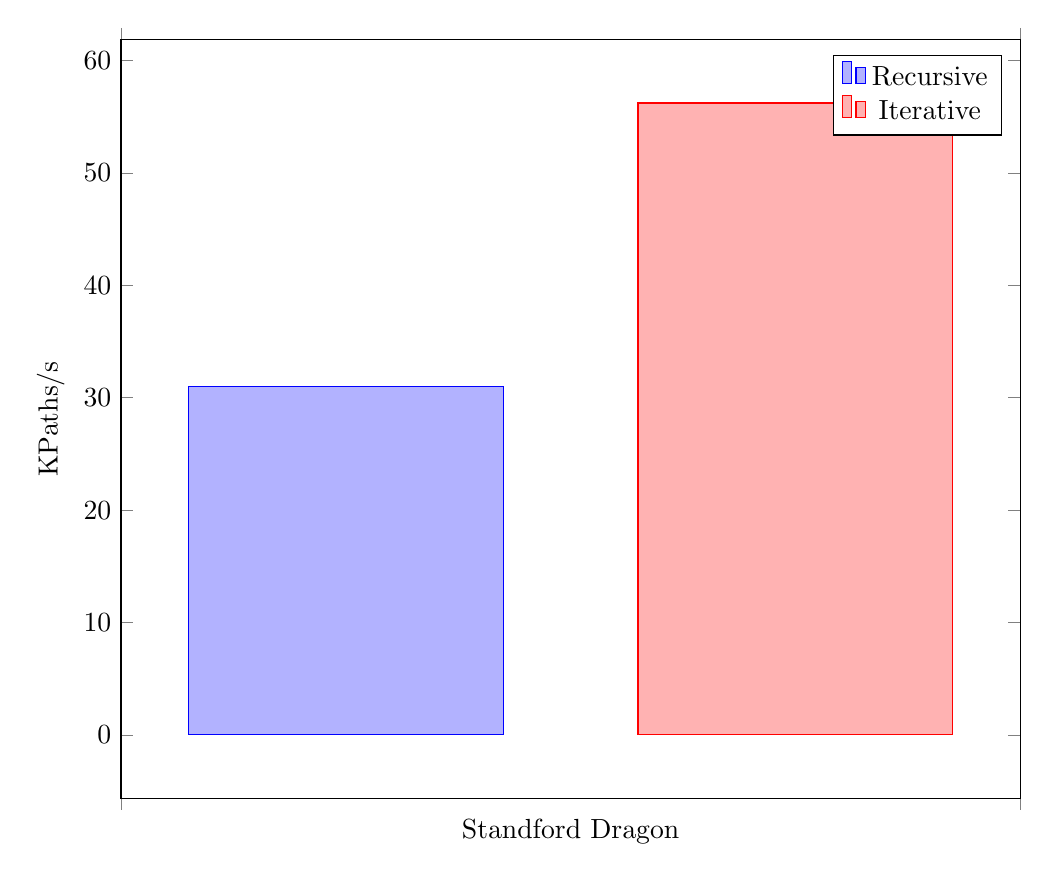
\begin{tikzpicture}
	\begin{axis}[
	x tick label style={
		/pgf/number format/1000 sep=},
	ylabel=KPaths/s,
	width=13cm,
	enlarge x limits=-1,
	ybar interval=0.7,
	symbolic x coords={Suzanne,Standford Bunny,Standford Dragon, test}
]
\addplot 
	coordinates {(Standford Dragon,31.03) (test,0)};
\addplot 
	coordinates {(Standford Dragon,56.23) (test,0)};
\legend{Recursive,Iterative}
\end{axis}
\end{tikzpicture}


	
\subsubsection{Comparación de heurísticas:}
	
Para justificar el uso de la heurística por superficie de área se muestra una ejecución de ambas heurísticas con tres modelos ampliamente utilizados en evaluaciones comparativas de computación gráfica:

\begin{itemize}
	
	\item Suzanne: 968 triángulos
	\item Standford Bunny: 4968 triángulos
	\item Standford Dragon: 871306 triángulos
	
\end{itemize}

\begin{figure}[H]
	\centering
  \begin{minipage}[b]{0.4\textwidth}
    \includegraphics[width=\textwidth]{bunny}
    \caption{Standford Bunny.}
  \end{minipage}
  \hfill
  \begin{minipage}[b]{0.4\textwidth}
    \includegraphics[width=\textwidth]{dragon}
    \caption{Standford Dragon.}
  \end{minipage}
\end{figure}

Esta evaluación ha sido llevada a cabo con los siguientes parámetros:

\code{BVH\_DEPTH = 20}, \code{BVH\_SAHBINS = 12}, \code{MAXBOUNCES = 5}, \code{SMOOTH\_SHADING = true}, 

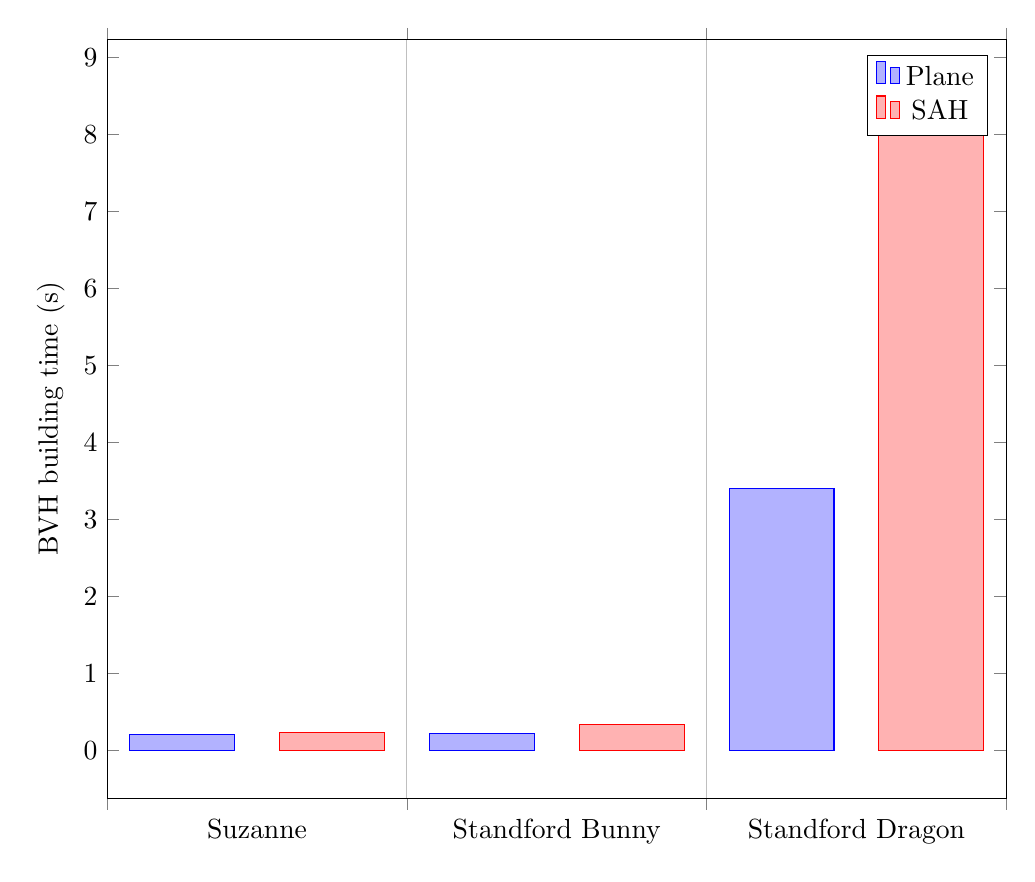
\begin{tikzpicture}
	\begin{axis}[
	x tick label style={
		/pgf/number format/1000 sep=},
	ylabel=BVH building time (s),
	width=13cm,
	enlarge x limits=-1,
	ybar interval=0.7,
	symbolic x coords={Suzanne,Standford Bunny,Standford Dragon, test}
]
\addplot 
	coordinates {(Suzanne,0.201) (Standford Bunny,0.215) (Standford Dragon,3.405) (test,3.405)};
\addplot 
	coordinates {(Suzanne,0.233) (Standford Bunny,0.342) (Standford Dragon,8.410) (test,3.405)};
\legend{Plane,SAH}
\end{axis}
\end{tikzpicture}
	
\subsection{Evaluación:}
	
Finalmente es necesario elegir los parámetros para \code{BVH\_DEPTH} y \code{SAH\_BINS}. Puesto que existen varios tipos de escenas con distintas geometrías, se va a dejar de lado cualquier tipo de enfoque analítico y se va a hacer uso de medidas en casos reales. Se procede a realizar una evaluación con distintos parámetros.
	
En el caso de la selección de \code{SAH\_BINS}, Indigo Wald propone 16 como límite \cite{wald2007fast} debido a la insustancial mejora de rendimiento para valores mayores. Esto se ha podido comprobar directamente en Eleven Renderer donde se ha llevado a cabo la construcción y recorrido de BVH para la escena "Standford Dragon" variando la cantidad de contenedores \autoref{fig:sahbins}. Se comprueba que la velocidad de recorrido se estanca para los valores 12-16, mientras que el tiempo de generación permanece lineal.

\begin{figure}[H]
\centering
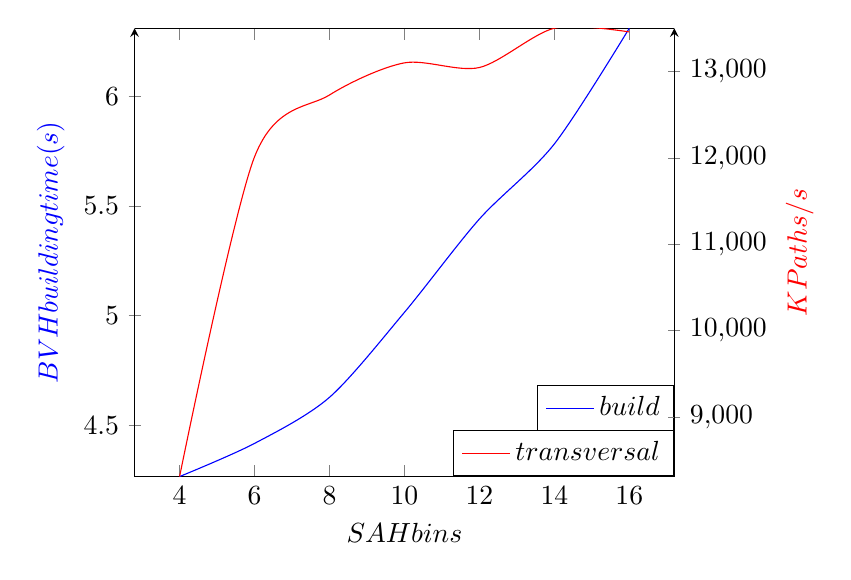
\begin{tikzpicture}
\label{fig:sahbins}
\begin{axis}[
    axis y line = left,
    xlabel = \(SAH bins\),
    ylabel = {\(\textcolor{blue}{BVH building time (s)}\)},
	legend style={at={(1,0.1)},anchor=south east},
	scaled y ticks=false
]

\addplot[smooth, blue]
coordinates{(4,4.267) (6, 4.418) (8, 4.628) (10, 5.015) (12, 5.440) (14, 5.782) (16, 6.309)};
\addlegendentry{\(build\)}
\end{axis}

\begin{axis}[
    axis y line = right,
	axis x line = none,
    xlabel = \(SAH bins\),
    ylabel = {\(\textcolor{red}{KPaths/s}\)},
	legend style={at={(1,0)},anchor=south east},
	scaled y ticks=false
]

\addplot [smooth, red]
coordinates{(4,8310) (6, 12012) (8, 12728) (10, 13100) (12, 13046) (14, 13501) (16, 13458)};
\addlegendentry{\(transversal\)}

\end{axis}
\end{tikzpicture}
\end{figure}